\documentclass{beamer}
\usetheme{default}
\usepackage[normalem]{ulem}

\begin{document}

\title{Team D Project Plan}
\author[C. Kolbeck, T. Wooster, E. Swanson, A. Miranda, J. Wagner, and F. Saldarini]{Cory Kolbeck, Tony Wooster, Erik Swanson, Adrien Miranda, Justin Wagner, and Federico Saldarini}
\institute[PSU]{
  Portland State University\\
  Department of Computer Science\\
  Portland, Oregon\\
}

\begin{frame}
  \titlepage
\end{frame}

\begin{frame}{Overview and Deliverables}
  We are to implement client libraries to provide asynchronous communication with a Burrow message queue server.

  The code for these libraries will reside on Github, and the sponsor will link to them from the main Burrow site. 
  Documentation will reside on the main Burrow website. 
\end{frame}

\begin{frame}{Assumptions}

  \begin{itemize}
  \item The code will be maintained by the OpenStack community
  \item The code will continue to reside on Github, or possibly be moved to launchpad
  \item Documentation will be hosted on burrow.openstack.org
  \item Authentication is outside the scope of this project
  \end{itemize}

\end{frame}

\begin{frame}{Restraints}

  \begin{itemize}
  \item Project will be distributed under the Apache2 license, and any libraries used must be compatible.
  \item All calls in to our library must be nonblocking.
  \item Maven will be used for Java builds.
  \item The Pandora autoconf macro set will be used for C builds.
  \item Minimal dependence on external libraries.
  \end{itemize}

\end{frame}

\begin{frame}{Plan Overview}
  The team will be split into two sub-teams of three.
  Erik, Justin, and Cory will create a library in Java.
  Tony, Fede and Adrian will create a library in C.

  \begin{enumerate}
  \item \sout{Meet with Eric Day to discuss project details}
  \item \sout{Decide on target languages}
  \item Create skeleton projects and integrate them with burrow continuous integration infrastructure
  \item Create blocking memory backends
  \item Research JSON and HTTP libraries
  \item Create blocking memory backend 
  \item Research asynchronous I/O
  \item Choose language appropriate callback mechanisms
  \item Write asynchronous memory backend
  \item Write asynchronous http backend
  \item Write unit tests (All through the above)
  \item Write functional tests
  \item Code Freeze
  \item \textit{Time Allowing} Write small projects which use our libraries in interesting ways.
  \end{enumerate}
\end{frame}

\begin{frame}{C Gantt Chart}
  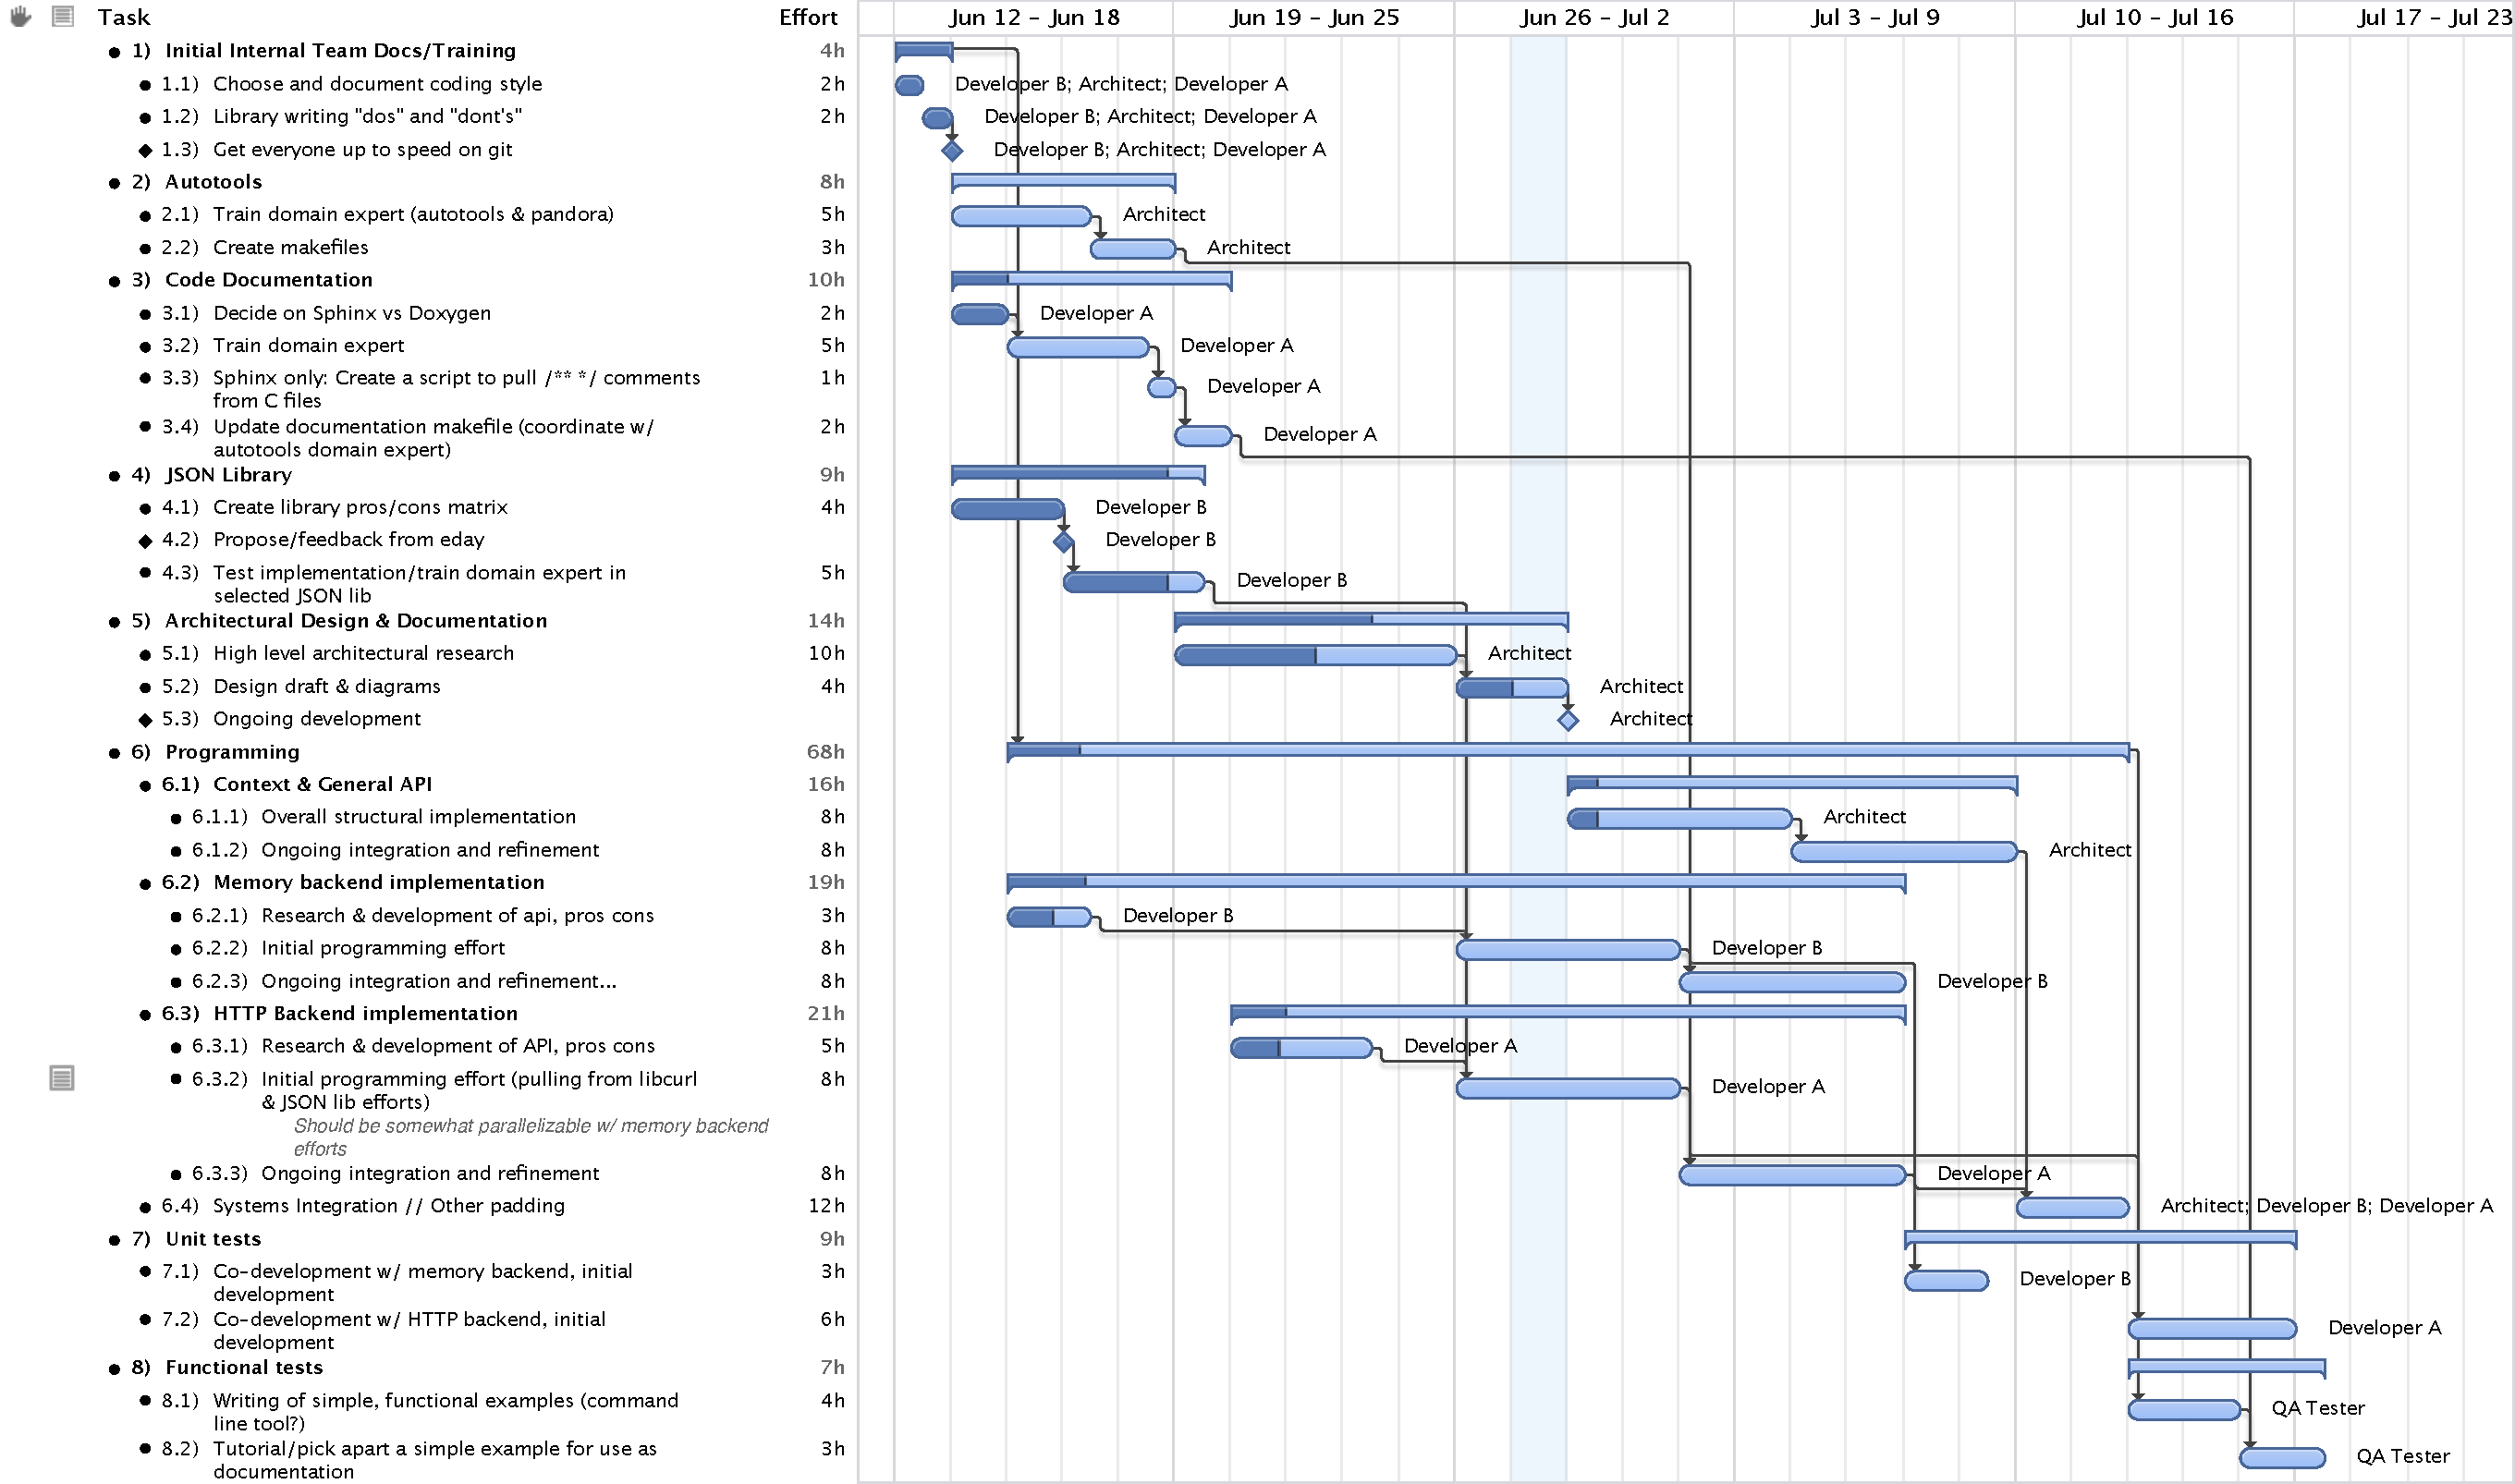
\includegraphics{C-Gantt.pdf}
\end{frame}

\begin{frame}{Java Gantt Chart}
  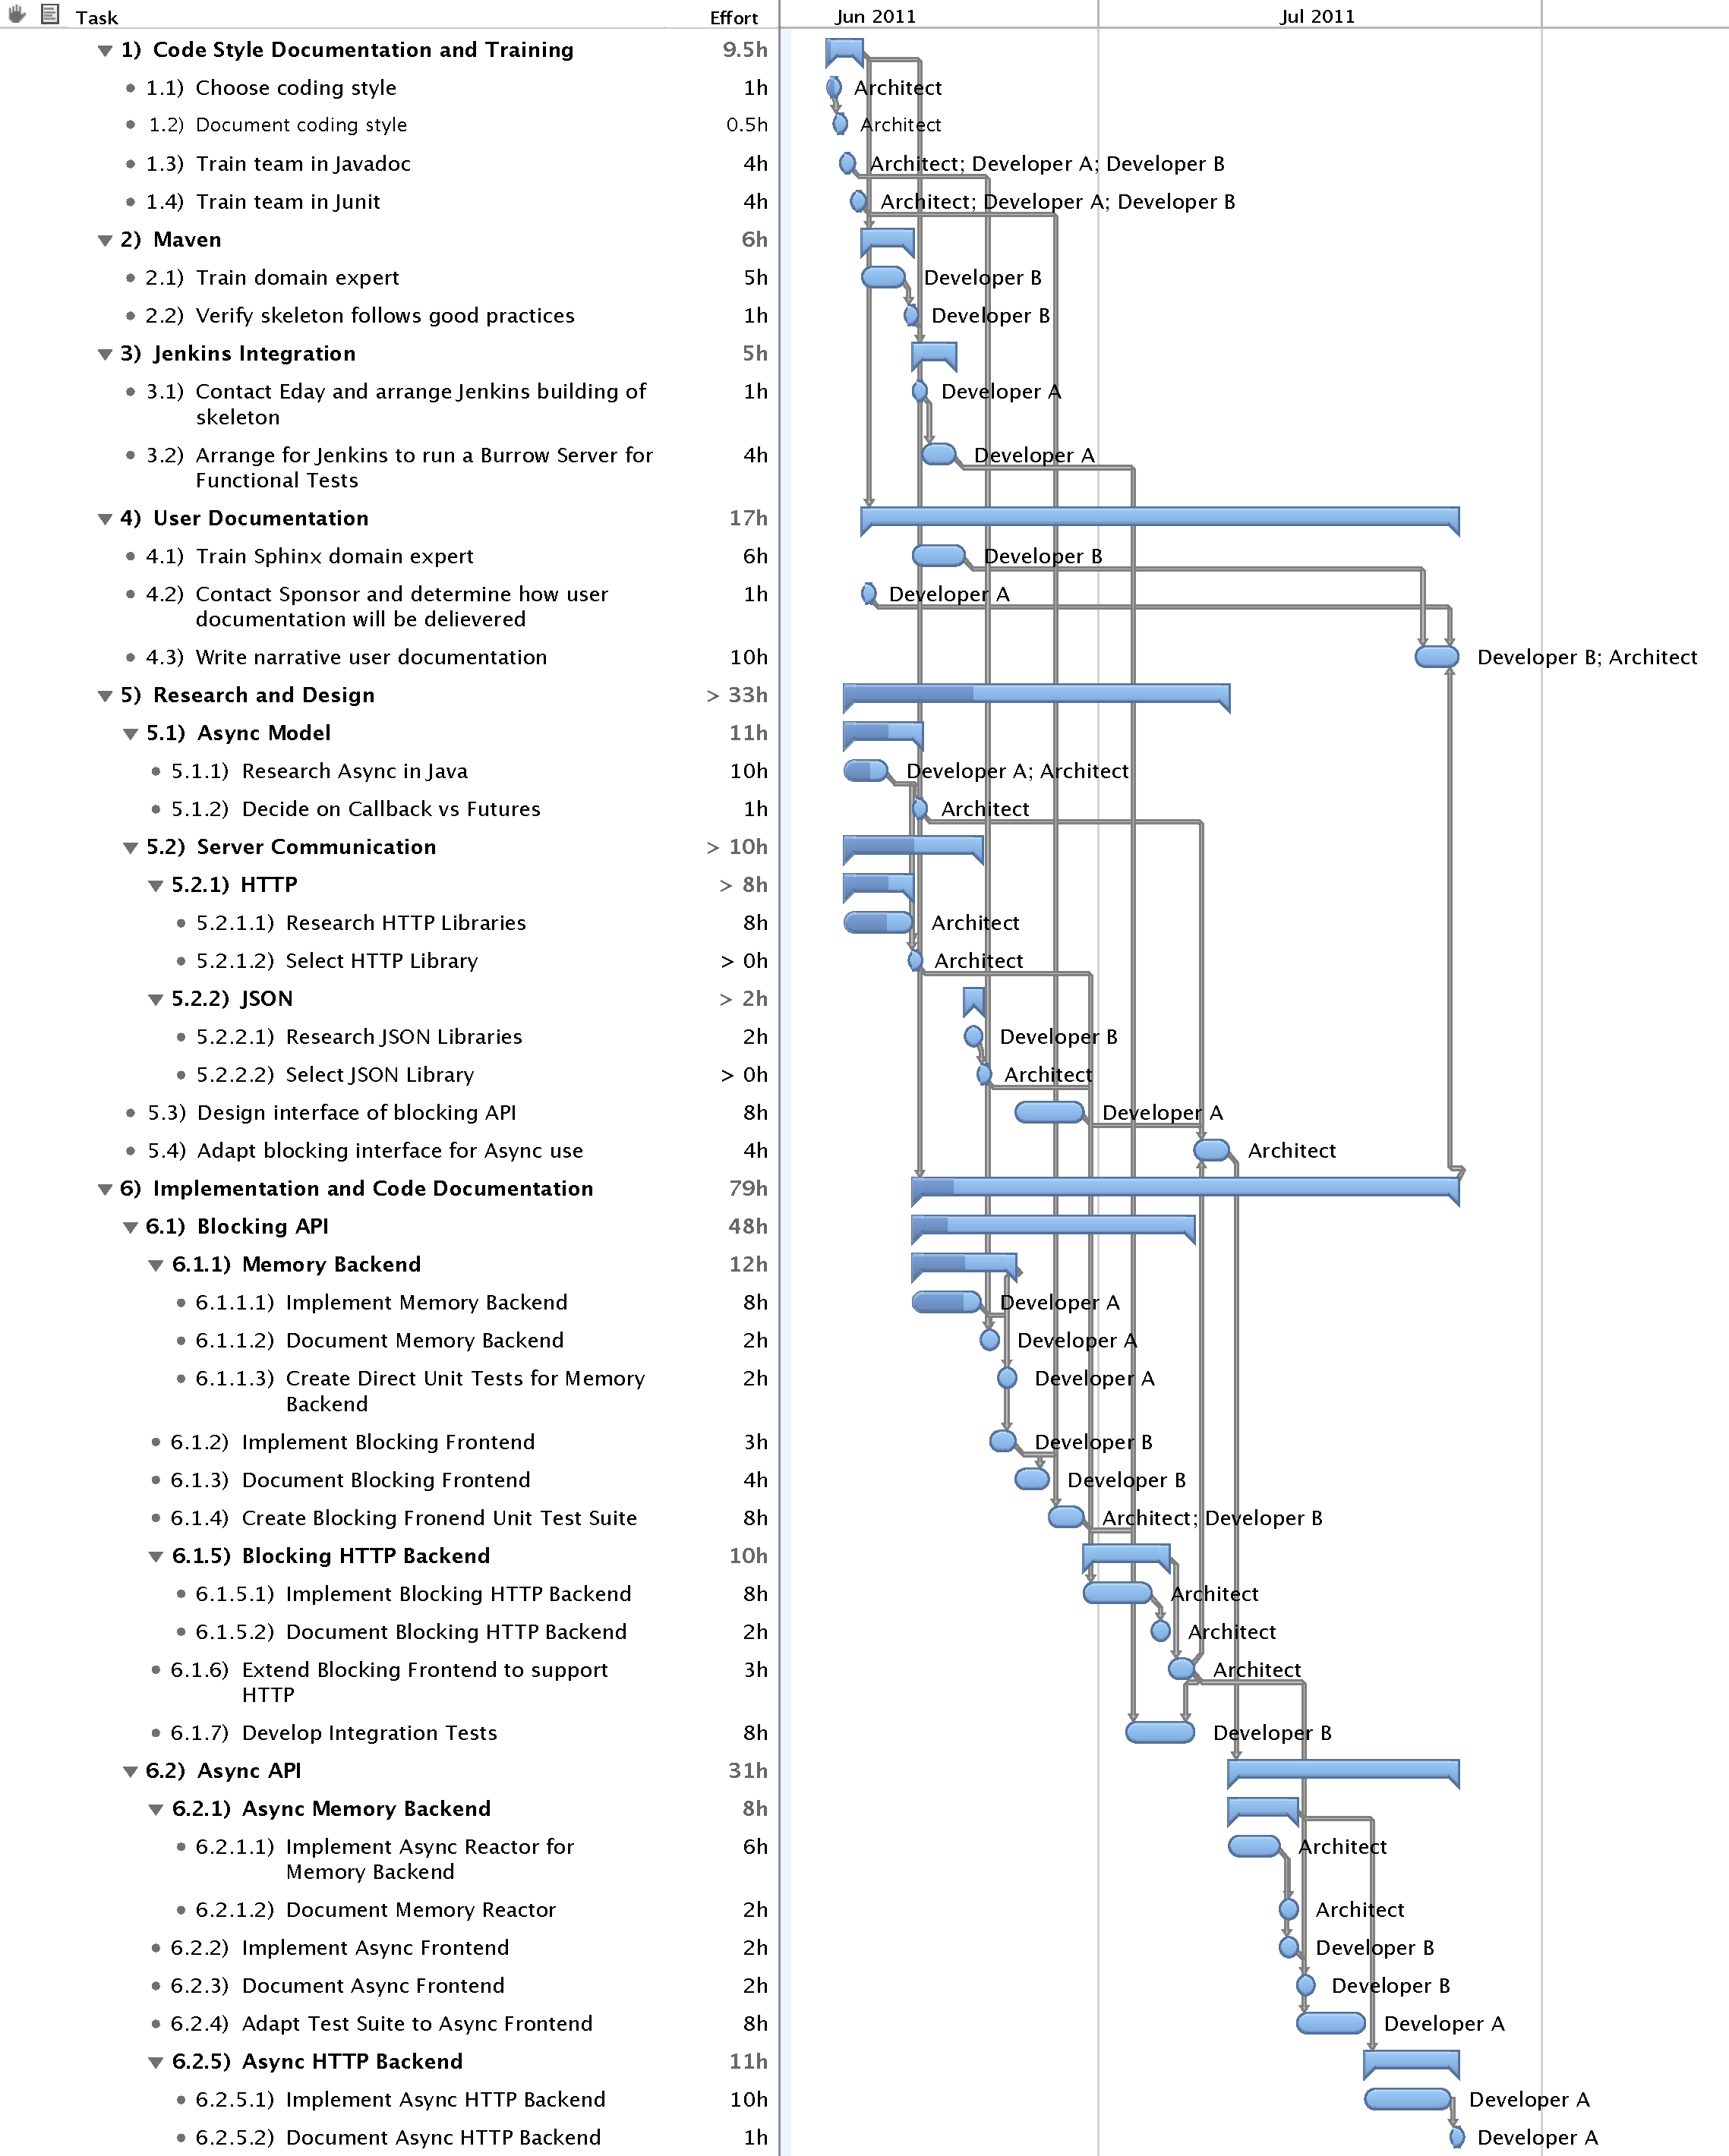
\includegraphics{Java-Gantt.pdf}
\end{frame}

\begin{frame}{Calendar}
  \begin{tabular}{|c|c|}
    \hline
  \end{tabular}

\end{frame}

%\begin{frame}{Meetings and Reviews}
%  \begin{itemize}
%  \item Jenkins Setup
%  \item Architecture review
%  \end{itemize}
%\end{frame}

\begin{frame}{Resource Identification}
  Time:
  \begin{tabular}{c|c}
    \emph{Name} & \emph{Available Hours/Week}\\ \hline
    Justin & 8-10\\ \hline
    Adrian & 8-10\\ \hline
    Tony & 8-10\\ \hline
    Erik & 10-15\\ \hline
    Federico & 10+\\ \hline
    Cory & 10-15\\ \hline
  \end{itemize}
\end{frame}

\begin{frame}{Configuration Management}
  Code will live in Github, using their systems for ticketing and bug reporting.  
  Should it become necessary, language leads will be in charge of resolving merge conflicts.
\end{frame}

\begin{frame}{Roles}
  \begin{tabular}{|c|c|c|}
    \hline
    \emph{Role} & \emph{Responsibility} & \emph{Name(s)}\\ \hline \hline
    Project Manager & Coordinate General Meetings, Designate Milestones, and Maintain Schedules & Cory\\ \hline
    Point of Contact & Maintain Communication between 
    Integration & Support Jenkins and Github issues & Cory\\ \hline 
    Java Lead & Architect Java library and Delegate Coding and Research Tasks & Erik\\ \hline
    C Lead & Architect C Library and Delegate Coding and Research Tasks & Tony\\ \hline
    Java Development & Implement Designs of Java Lead & Cory, Justin, Erik\\ \hline
    C Development & Implement Designs of C Lead & Adrien, Federico, Tony\\ \hline
    System Support & Maintain Shared Machines & Cory\\ \hline
    Unit Testing & Code Unit Tests for Every Function & Everyone\\ \hline
    Functional Testing & Create Functional Tests for Each Language & To be delegated by appropriate lead\\ \hline
    Memory Backend Creation & Create Memory Backend for Testing & To be delegated by appropriate lead\\ \hline
    API Documentation & Write Language Specific Documentation & To be delegated by appropriate lead\\ \hline
    General Documentation & Create a Language Agnostic Guide to Coding Burrow Clients & ?Tony?\\ \hline
  \end{tabular}
\end{frame}

\begin{frame}{Risk Management}
  \begin{itemize}
  \item Risk: Team member drops out\\
    Consequence: Fewer man-hours available\\
    Mitigation: Scheduling as if we have 2 weeks fewer\\
  \item Risk: Architect drops out\\
    Consequence: Possible loss of grand plan\\
    Mitigation: Documentation, regular meetings to keep team members in the loop\\
  \item Risk: API Change mid-project\\
    Consequence: Project may need re-architecting\\
    Mitigation: Modular design\\
  \end{itemize}
\end{frame}

\begin{frame}{QA and Deployment}
  Unit and regression testing will be ongoing using Burrow's existing Jenkins continuous integration system.
  
  Functional testing will take place in the weeks leading up to code freeze.

  Deployment will consist of linking to our existing Github repositories (or possibly official forks)
  from burrow.openstack.org.  Documentation will be pulled from Github by our sponsor for inclusion in the Burrow wiki.
\end{frame}

\end{document}
